\documentclass[20pt,margin=1in,innermargin=-4.5in,blockverticalspace=-0.25in]{tikzposter}
\geometry{paperwidth=42in,paperheight=30in}
\usepackage[utf8]{inputenc}
\usepackage{amsmath}
\usepackage{amsfonts}
\usepackage{amsthm}
\usepackage{amssymb}
\usepackage{mathrsfs}
\usepackage{graphicx}
\usepackage{adjustbox}
\usepackage{enumitem}
\usepackage[backend=biber,style=numeric]{biblatex}
\usepackage{emory-theme}

\usepackage{color}
\usepackage{algorithm}  
\usepackage{algorithmic}  

\usepackage{mwe} % for placeholder images

\newcommand{\expection}[1]{\mathbb{E} \, #1}
\newcommand{\argmin}[1]{\underset{#1}{\operatorname{arg}\operatorname{min}}\;}
\newtheorem{theorem}{Theorem}
%\addbibresource{refs.bib}

% set theme parameters
\tikzposterlatexaffectionproofoff
\usetheme{EmoryTheme}
\usecolorstyle{EmoryStyle}

\title{Drug Sensitivity Estimation Based on Adaptive Empirical Conditional Expectation}
\author{FAN Min\textsuperscript{$\dagger$}}
\institute{\textsuperscript{$\dagger$}Department of Mathematics, Hong Kong University of Science and Technology}
\titlegraphic{
\includegraphics[width=0.15\textwidth]{HKUST.eps}}

% begin document
\begin{document}
	\maketitle
	\centering
	\begin{columns}
		\column{0.32}
		
		\block{Abstract}{
			Predicting drug sensitivity to specific cancer cell line is an essential part for personalized cancer therapy. Traditional machine learning algorithms do not perform very well in this scenario. The reasons probably is because the features of cancer cell lines are binary and the number of training samples is limited due to the high cost of experiments. In this work, we proposed a new model called Adaptive Empirical Conditional Expectation(AECE) from the perspective of probability and statistics. The model achieved the highest performance among traditional machine learning algorithms, like Support Vector Regression(SVR), Random Forest(RF), Gradient Boosting(GB), Multilayer Perceptron(MLP). Moreover, the model is tuning-free, capable to candle missing features and does not need to assume training and test cell lines are from the same distribution.
			\vspace{1em}
		}
		
		\block{Problem Setting}{
			In training data, there are 542 cancer cell lines. Each cell line has 60 binary features, $ X = [x_{1}, \dots , x_{60}] \in \left\lbrace 0, 1\right\rbrace ^{60} $, which correspond to the mutation status of 60 cancer genes. The drug sensitivity of cancer cell lines to the specific drug, Afatinib, is measured by IC50s which is expected to be smaller for high sensitive cell lines and larger for low sensitive cell lines. Roughly speaking, the negative values of logarithmic IC50 indicate the cell line is sensitive to the drug and positive values indicate the resistance to the drug. In testing data, we need to predict IC50s of 100 cancer cell lines with the mutation status of 60 cancer genes.
			\vspace{1em}
		}
		\block{Empirical Conditional Expectation}{
			Given feature $ X $, IC50, denoted as $ y(X) $, can be regarded as a random variable (r.v.) due to the randomness in biology. In testing data, the estimator (prediction) of IC50 is also a r.v., denoted as $ \hat{y}(X) $, since estimator is a function of IC50s in training data, which are also r.v.s.
			\vspace{1em}
			
			\textbf{In practice}, we minimize mean squared error (MSE):
			
			\begin{align*}
				\text{MSE} &:= \frac{1}{n}\sum_{i=1}^{n}( \hat{y}(X_{i}) - y(X_{i}) )^{2}\\
				&= \sum_{j=1}^{t} \frac{n_{j}}{n} \left\lbrace {\color{red} \frac{1}{n_{j}} \sum_{i=1}^{n_{j}} [ \hat{y}(X_{j}) - y(X_{j}) ]^{2} } \right\rbrace 
			\end{align*}
			
			\textbf{In theory}, by law of large number, minimizing MSE is equivalent to minimize following:
			\begin{equation*}
				\text{Overall Error} :=\mathbb{E}_{X \sim p_{test}}{[ {\color{red} \mathbb{E}_{y}(\hat{y}(X) - y(X))^{2}}  ]}.
			\end{equation*}
			One essential assumption of most machine learning algorithms is $ p_{test} = p_{train} $. However, it may not hold sometimes, like personalized cancer therapy of specific patient. We can see it later that our model can also tackle this case.
			\vspace{1em}
			
			{\color{red} Theorem}\hspace{1em}Suppose $ \expection{X^{2}} < \infty $ and $ \mathcal{F} $ is a $ \sigma $-algebra,
			\begin{equation*}
				\expection{( X | \mathcal{F} )} = \argmin{Y \in \mathcal{F}} \expection{(X-Y)^{2}}.
			\end{equation*}
			It tells us that $ \expection{( X | \mathcal{F} )} $ is the best guess of $ X $ given the information $ \mathcal{F} $. We can implement the same idea to minimize the red part above, that is, $ \mathbb{E}_{Y}(\hat{y}(X) - y(X))^{2} $.
		}
		
		\column{0.36}
		\block{}{
			First, we construct $ \mathcal{F}_0 \subset \mathcal{F}_1 \subset ... \subset \mathcal{F}_{60} $ by computing p-values of features. In particular, for feature $ i $, we can test the hypothesis using T-Test
			\begin{equation*}
				H_0: \mathbb{E}(y|X_i=0) = \mathbb{E}(y|X_i=1) \quad \mathrm{versus} \quad
				H_1: \mathbb{E}(y|X_i=0) \ne \mathbb{E}(y|X_i=1).
			\end{equation*}
			
			\begin{tikzfigure}[P-values]
				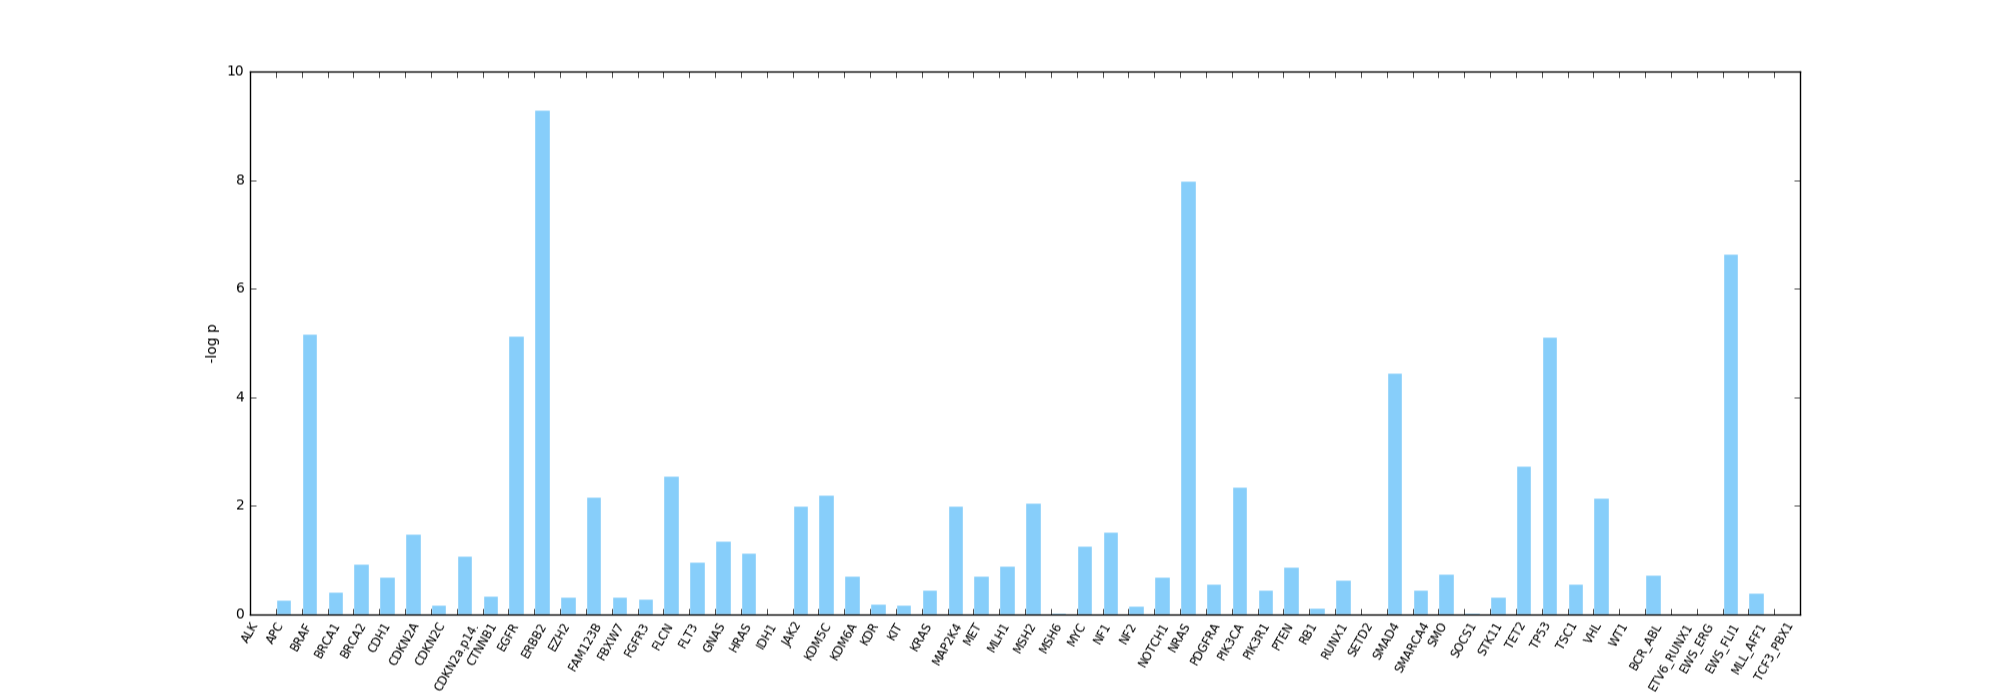
\includegraphics[width=0.7\linewidth]{pvalues.png}
			\end{tikzfigure}
		
			And we sort features as p-value descending order. $ \mathcal{F}_k $ is the feature space discarding last $ 60-k $ insignificant features. Then given specific feature $ \bar{X} $we can approximate $ \expection{( y(X = \bar{X}) | \mathcal{F}_k )} $ by averaging $ y(X) $ of training samples with the same feature of $ \bar{X} $ in $ \mathcal{F}_k $, called empirical conditional expectation.
			\vspace{1em}
			
			For example, in the figure below, $ \mathcal{F}_2 $ is the feature space containing feature 1 and 2. We need to predict IC50s of the sample in last row. $ \expection{( y(X = \bar{X}) | \mathcal{F}_2 )} = \frac{1}{2} (2.1 + 2.2) = 2.15$.
			\begin{tikzfigure}[Example of Empirical Conditional Expectation]
				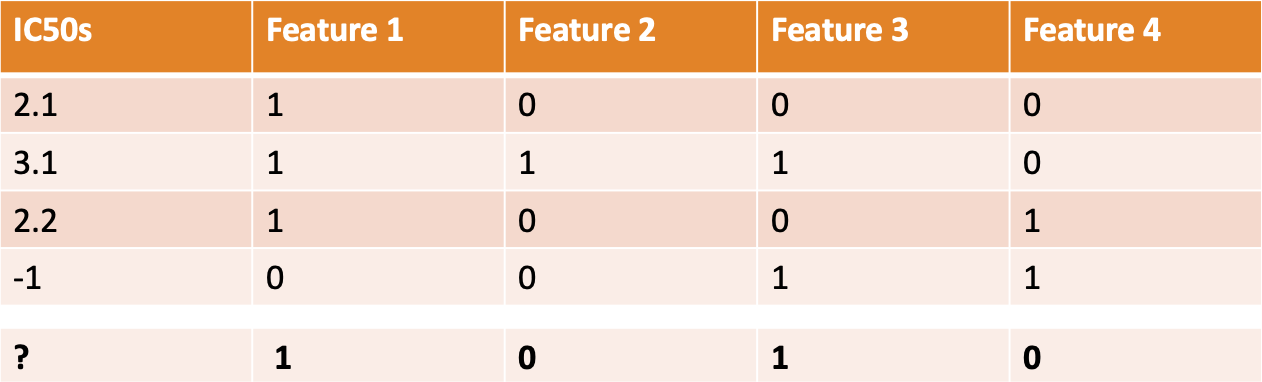
\includegraphics[width=0.5\linewidth]{example}
			\end{tikzfigure}
			
			The larger $ k $ is, the more information $ \mathcal{F}_k $ contains and the more accurate $ \expection{( y(X = \bar{X}) | \mathcal{F}_k )} $ is. So we can propose Vanilla Empirical Conditional Expectation(ECE) below.
			
			\begin{tikzfigure}
				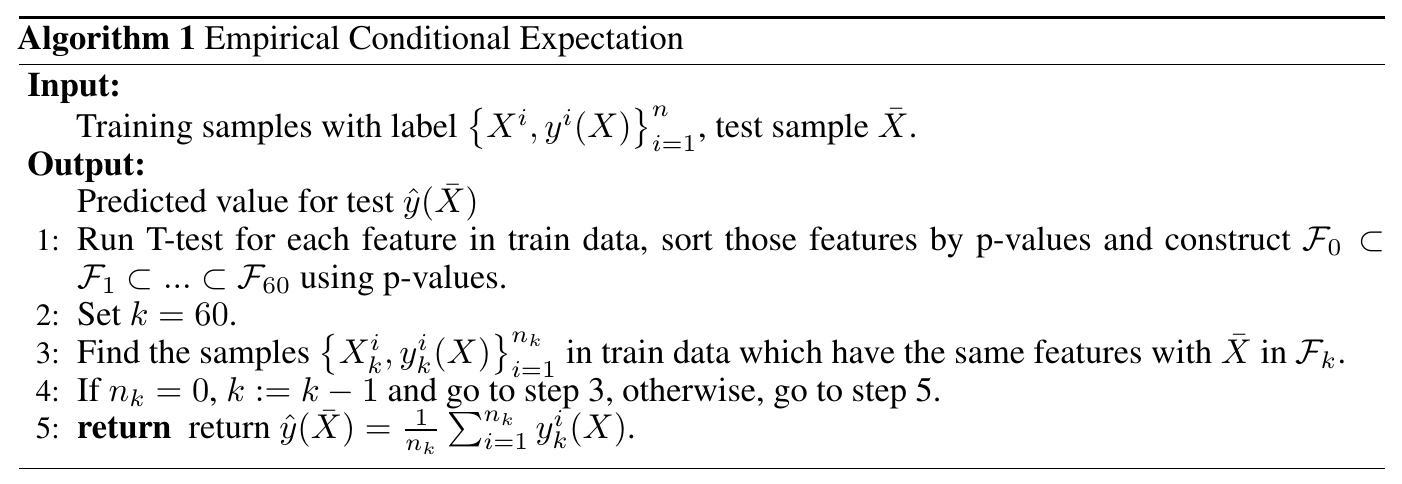
\includegraphics[width=0.85\linewidth]{algorithm1}
			\end{tikzfigure}
	    }
			
		\block{Adaptive Empirical Conditional Expectation}{
			\begin{align*}
				\mathbb{E}_{y} (\hat{y}(X) - y(X))^{2} &= \mathbb{E}_{y} ( \hat{y}(X) - \expection{\hat{y}(X)} )^{2} + \mathbb{E}_{y} ( \expection{\hat{y}(X)} - \expection{y(X) )^{2}}  + \expection{( \expection{y(X) - y(X) )^{2}} }\\
				&= \mathrm{Var}(\hat{y}(X)) + \mathrm{Bias}^2(\hat{y}(X)) + \mathrm{Var}(y(X)).
			\end{align*}
			Last term $ \mathrm{Var}(y(X)) $ caused by randomness in biology is intrinsic and we can only minimize the first two terms. If $ \hat{y}(\bar{X}) = \frac{1}{n_k} \sum_{i = 1}^{n_k} y_k^i(X) $, intuitively, the larger $ k $ is, the smaller $ \mathrm{Var}(\hat{y}(X) $ is and the larger $ \mathrm{Bias}^2(\hat{y}(X)) $. So we have to make a trade-off on $ k $ to minimize the sum ot them.
			\vspace{1em}
			
			$ \mathrm{Bias}^2(\hat{y}(X)) $: $ \expection{y(X)} $ is approximated by the average of returns in algorithms 1 by bootstrapping 50 times, denoted as $ \hat{\mathbb{E}}y(X) $. Given $ k $, $ \expection{\hat{y}(X)} $ is approximated by the average of empirical conditional expectation with $ \mathcal{F}_k $ by bootstrapping 50 times, denoted as $ \hat{\mathbb{E}}\hat{y}_k(X) $. Hence, $ \mathrm{Bias}^2(\hat{y}(X)) $ can be approximated by $ (\hat{\mathbb{E}}\hat{y}_k(X) - \hat{\mathbb{E}}y(X))^{2} $, denoted as $ \hat{\mathrm{Bias}}^2(\hat{y}_k(X)) $.
		}
		
		\column{0.32}
		\block{}{
			$ \mathrm{Var}(\hat{y}(X) $: Given $ k $, $ \mathrm{Var}(\hat{y}(X) $ is approximated by the variance of empirical conditional expectation with $ \mathcal{F}_k $ by bootstrapping 50 times, denoted as $ \hat{\mathrm{Var}}(\hat{y}_k(X)) $.
			\vspace{0.1em}
			
			$ k $ is decreasing from 60. Adopting early stopping idea, we choose the largest $ k $ such that $ \hat{\mathrm{Bias}}^2(\hat{y}_k(X)) + \hat{\mathrm{Var}}(\hat{y}_k(X)) < \hat{\mathrm{Bias}}^2(\hat{y}_{k-1}(X)) + \hat{\mathrm{Var}}(\hat{y}_{k-1}(X))$.
			\vspace{1em}
			
			Adaptive Empirical Conditional Expectation(AECE) is stated as below.
			\begin{tikzfigure}
				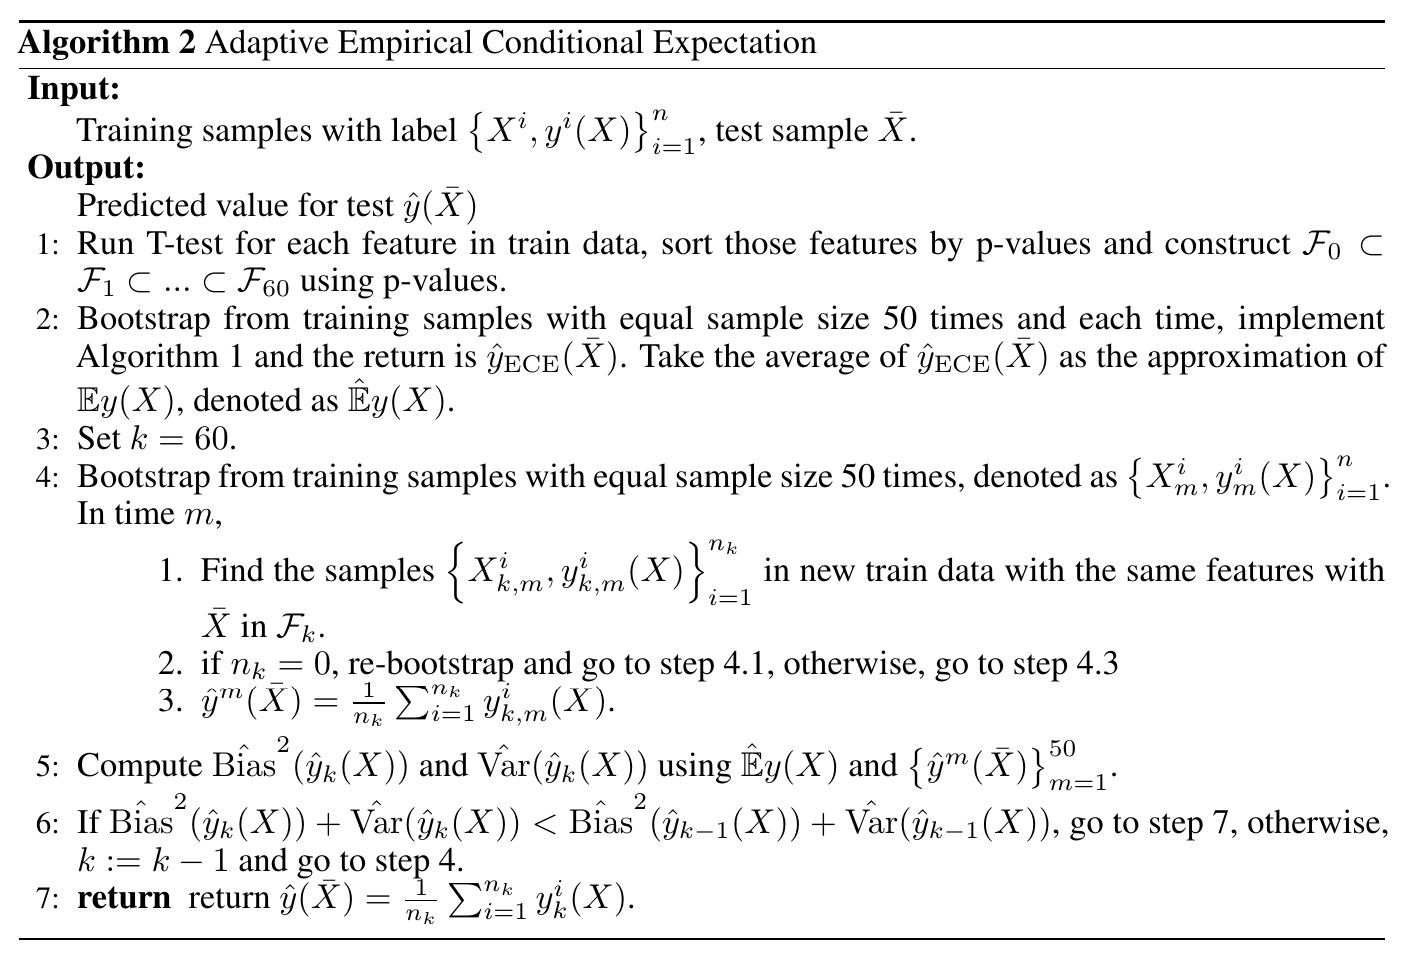
\includegraphics[width=0.9\linewidth]{algorithm2}
			\end{tikzfigure}
		}
		
		
		\block{Result}{
			AECE achieved the highest performance in the competition and the MSE is only 3.04446.
			
			\begin{tikzfigure}
				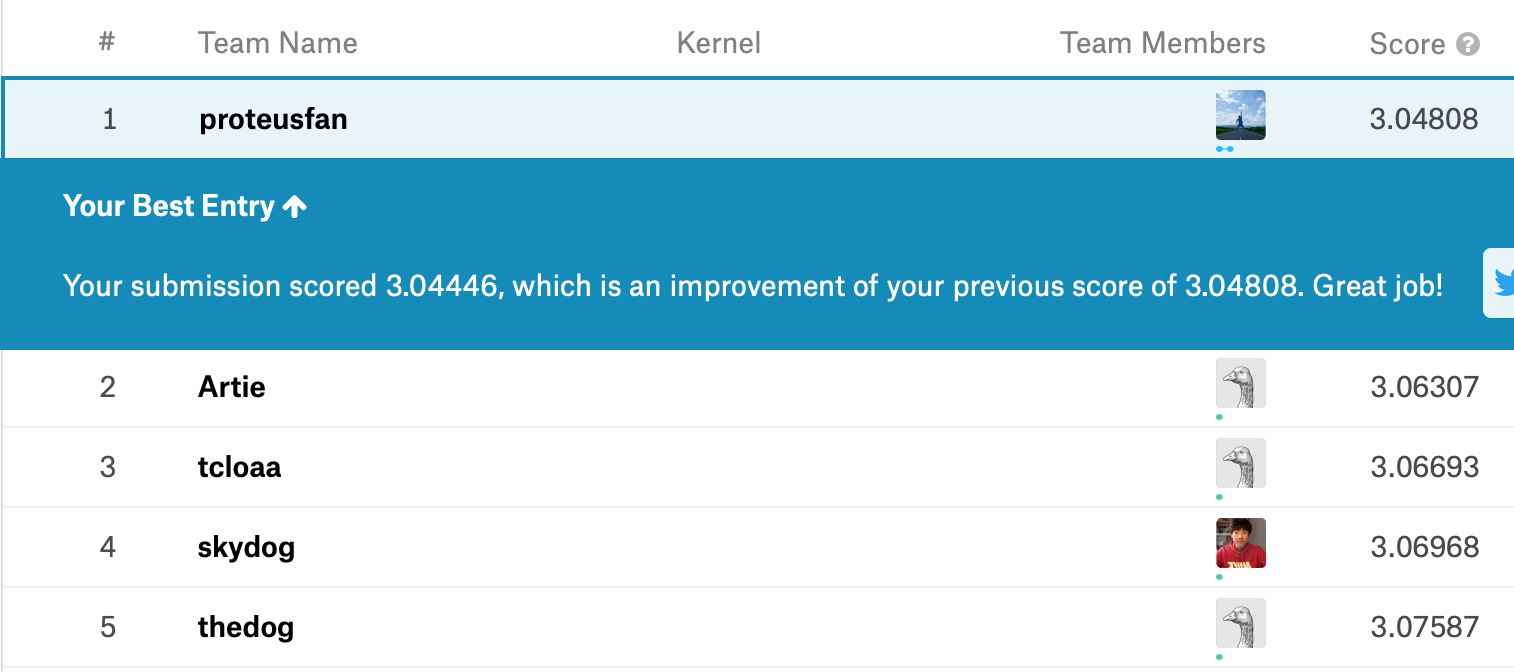
\includegraphics[width=0.5\linewidth]{result}
			\end{tikzfigure}
			
		}
		
		\block{Discussion}{
			{\color{red} Advantage}: 
			\begin{itemize}
				\item	capable to candle missing features
				\item	tuning-free
				\item 	capable to do prediction of samples with specific feature($ p_{train} \neq p_{test} $)
			\end{itemize}
		
			{\color{red} Disadvantage}: 
			\begin{itemize}
				\item time-consuming in finding appropriate $ k $ 
			\end{itemize}
		
			{\color{red} Potential Improvement}: 
			\begin{itemize}
				\item use local FDR to replace t-test
				\item approximate $ \mathrm{Var}(\hat{y}(X)) $ and $ \mathrm{Bias}^2(\hat{y}(X)) $ more accurate
				\item speed up the algorithm
			\end{itemize}
		}
		
%		\block{Remarks}{
%			
%		}
		
%		\block{Acknowledgements}{
%			
%		}
	
%		\block{References}{
%			\vspace{-1em}
%			\begin{footnotesize}
%				\printbibliography[heading=none]
%			\end{footnotesize}
%		}
		
	\end{columns}
\end{document}